\documentclass[a4paper]{article}
\setlength{\columnsep}{10pt}                                                                    %兩欄模式的間距
\setlength{\columnseprule}{0pt}                                                                %兩欄模式間格線粗細

\usepackage{fullpage} % Package to use full page
\usepackage{parskip} % Package to tweak paragraph skipping
\usepackage{tikz} % Package for drawing
\usepackage{amsmath}
\usepackage{hyperref}
\usepackage{fancyhdr}	
\usepackage[CheckSingle, CJKmath]{xeCJK}
\usepackage{amsmath, courier, listings, fancyhdr, graphicx}
\setCJKmainfont{Source Han Sans TC}

\usepackage{caption}
\usepackage{subcaption}
\usepackage{placeins}

\title{線性代數作業1}
\author{0516009 吳宗達}
\date{2016/11/16}

\begin{document}
\large
\fancyhead[R]{交通大學105學年度線性代數作業}
\maketitle

\section{背景介紹}
給你 n 個點對 (xi,yi) 和 m 個方程式 Fk(x),找出一組係數xhead使得sumk=0~m(Fk(xi)) 與 yi 要盡量靠進,也就是delta = sumi=1~n( sumk=0~m(Fk(xi))-yi ) / n 要最小化

\section{程式說明}
以 matlab2016 來實做程式,讀入一筆資料

\section{執行結果}
\subsection{測試1}
以 Fk = (...........) 逼近
\begin{figure}[!htbp]
	\centering
	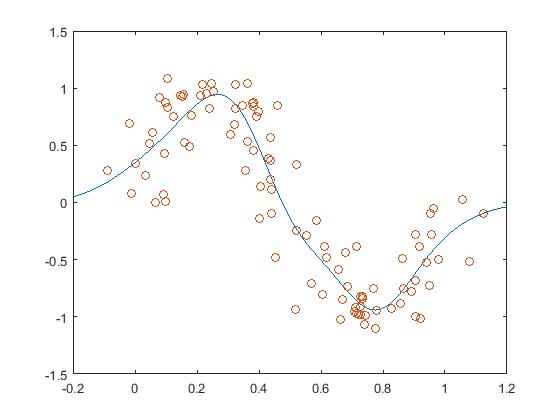
\includegraphics[width=.8\linewidth]{Figure11.jpg}
	\captionof{figure}{delta = 0.www}
\end{figure}
\begin{figure}[!htbp]
	\centering
	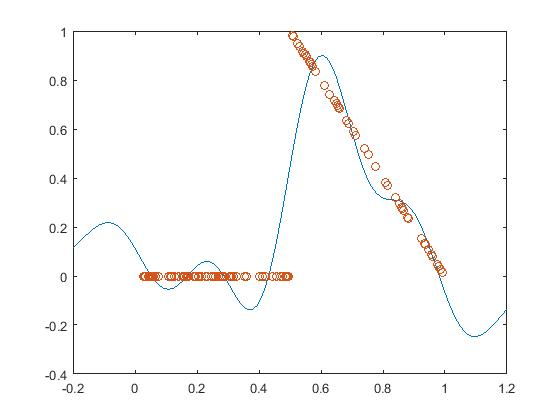
\includegraphics[width=.8\linewidth]{Figure12.jpg}
	\captionof{figure}{delta = 0.www}
\end{figure}
\newpage
\subsection{測試2}
以 Fk = (...........) 逼近
\begin{figure}[!htbp]
	\centering
	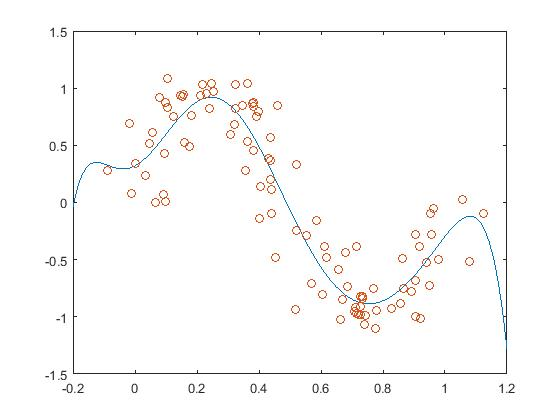
\includegraphics[width=.8\linewidth]{Figure21.jpg}
	\captionof{figure}{delta = 0.www}
\end{figure}
\begin{figure}[!htbp]
	\centering
	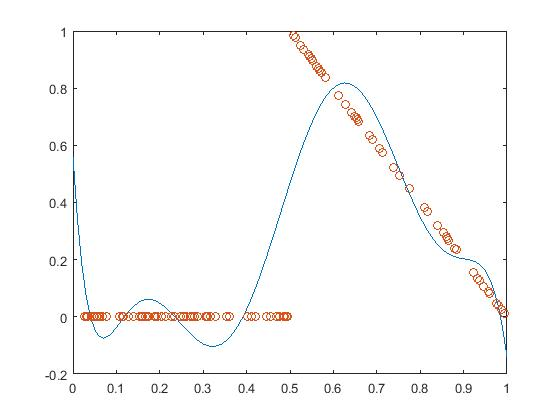
\includegraphics[width=.8\linewidth]{Figure22.jpg}
	\captionof{figure}{delta = 0.www}
\end{figure}
%\newpage
\section{結論}

\section{連結}

\end{document}
